\section{The Elements of tkz code}

To work with this package, you need some knowledge of \LATEX\ and of \TIKZ.

In this section, we look at the \code{rules} and \code{symbols} used to create a figure with \tkzname{\tkznameofpack}.

\subsection{Objects and language}

 The primitive objects are points. You can refer to a point at any time with the name given when it was defined (it is possible to give it another name later).

New points are obtained with macros. The names of the \tkzname{\tkznameofpack} macros begin with \code{tkz}. There are four main categories, starting with:
|\tkzDef...| |\tkzDraw...| |\tkzMark...| and |\tkzLabel...|. 
The points used are passed as arguments between parentheses, while the points created are given between braces.

The code of a figure is placed in a \tkzimp{tikzpicture} environment.


Contrary to \TIKZ, a macro must not end with “;”. We thus lose the important notion of \tkzimp{path}. However, you can place some \TIKZ\ code between the \tkzname{\tkznameofpack} macros.
 

In the first category, |\tkzDefPoint| defines fixed points; it will be studied in detail later. Here we look at the macro |\tkzDefTriangle|.

This macro associates a third point with a pair of points, in order to define a certain triangle: |\tkzDefTriangle(A,B)|. The point obtained is referenced |tkzPointResult|, and you can choose another reference, for example with |\tkzGetPoint{C}|.

|\tkzDefTriangle[euclid](A,B) \tkzGetPoint{C}|

Parentheses are used to pass arguments: in |(A,B)|, $A$ and $B$ are the points from which a third one will be defined. In |{C}|, braces are used to retrieve the new point.

To choose a type of triangle among the following:
  |equilateral|,  |isosceles right|, |half|, |pythagoras|, |school|, |golden or sublime|, |euclid|, |gold|, |cheops|...
 and |two angles|, you just give the option between square brackets, for example:
 
\begin{minipage}{0.5\textwidth}
  \begin{tikzpicture}[scale=.5]
  \tkzDefPoints{0/0/A,8/0/B}
  \foreach \tr in {golden, equilateral}
  {\tkzDefTriangle[\tr](A,B) \tkzGetPoint{C}
  \tkzDrawPoint(C)
  \tkzLabelPoint[right](C){\tr}
  \tkzDrawSegments(A,C C,B)}
  \tkzDrawPoints(A,B)
  \tkzDrawSegments(A,B)
   \tkzLabelPoints(A,B)
  \end{tikzpicture}
\end{minipage}
\begin{minipage}{0.5\textwidth}
  \begin{tkzexample}[code only,small]
    \begin{tikzpicture}[scale=.5]
    \tkzDefPoints{0/0/A,8/0/B}
   \foreach \tr in {golden, equilateral}
    {\tkzDefTriangle[\tr](A,B) \tkzGetPoint{C}
    \tkzDrawPoint(C)
    \tkzLabelPoint[right](C){\tr}
    \tkzDrawSegments(A,C C,B)}
    \tkzDrawPoints(A,B)
    \tkzDrawSegments(A,B)
    \tkzLabelPoints(A,B)
    \end{tikzpicture}
  \end{tkzexample}
\end{minipage}

\subsection{Notations and conventions}

I deliberately chose French geometric conventions, and some personal ones, to describe the objects represented. The objects defined and drawn by \tkzname{\tkznameofpack} are points, lines and circles in a plane. They are the primary objects of Euclidean geometry, from which we construct figures.

According to \tkzimp{Euclid}, these figures only illustrate pure ideas produced by our mind.
Thus a point has no dimension and therefore no real existence. In the same way, a line has no width and therefore no existence in the real world. The objects we consider are only representations of ideal mathematical objects. \tkzname{\tkznameofpack} follows the steps of the ancient Greeks to obtain geometric constructions with ruler and compass.

Here are the notations used:

\begin{itemize}
\item Points are represented either by a small disc or by the intersection of two lines (two straight lines, a straight line and a circle, or two circles). In the second case, the point is represented by a cross.

\begin{tkzexample}[latex=6cm, small]     
  \begin{tikzpicture}       
    \tkzDefPoints{0/0/A,4/2/B}       
    \tkzDrawPoints(A,B)       
    \tkzLabelPoints(A,B)     
  \end{tikzpicture}    
\end{tkzexample}

or else

\begin{tkzexample}[latex=6cm, small]     
  \begin{tikzpicture}       
    \tkzSetUpPoint[shape=cross, color=red]       
    \tkzDefPoints{0/0/A,4/2/B}       
    \tkzDrawPoints(A,B)       
    \tkzLabelPoints(A,B)     
    \end{tikzpicture}    
    \end{tkzexample}  

Once a point exists, we can give it a label, which is a capital letter of the Latin alphabet (with some exceptions) such as $A$, $B$ or $C$. For example:
\begin{itemize}
\item $O$ is a center for a circle, a rotation, etc.;
\item $M$ is a midpoint;
\item $H$ is the foot of an altitude;
\item $P'$ is the image of $P$ by a transformation.
\end{itemize}

Note that the reference name of a point in the code may differ from the label that designates it in the text: we can define a point A and give it the label $P$. The style is also different: the point A is labelled $A$.

\begin{tkzexample}[latex=6cm, small]     
  \begin{tikzpicture}       
    \tkzDefPoint(0,0){A}       
    \tkzDrawPoints(A)       
    \tkzLabelPoint(A){$P$}     
  \end{tikzpicture}    
\end{tkzexample}

Exceptions: some points, such as the midpoints of the sides of a triangle, share a property, so their names also share a common letter. We designate these points by $M_a$, $M_b$ and $M_c$, or $M_A$, $M_B$ and $M_C$.

In the code, these points are referred to as M\_A, M\_B and M\_C.

Another exception concerns intermediate construction points, which are not labelled. They are often designated by a lowercase letter in the code.

\item Segments are designated by their two endpoints in square brackets: $[AB]$.

\item In Euclidean geometry, a straight line is defined by two points: $A$ and $B$ define the line $(AB)$. We can also name a line with a Greek letter, $(\delta)$ or $(\Delta)$, or with a lowercase letter such as $d$ or $d'$.

\item A ray (half-line) is written $[AB)$.

\item Relations between lines: if $(AB)$ and $(CD)$ are perpendicular we write $(AB) \perp (CD)$, and if they are parallel we write $(AB) \parallelslant (CD)$.

\item The lengths of the sides of the triangle $ABC$ are $AB$, $AC$ and $BC$. Numbers are also designated by lowercase letters, so we write $AB=c$, $AC=b$ and $BC=a$. The letter $a$ is also used for an angle; $r$ is often used for a radius, $d$ for a diameter or a distance, $l$ for a length.

\item Polygons are designated by their vertices: $ABC$ is a triangle, $EFGH$ a quadrilateral.

\item Angles are generally measured in degrees (for example $60^\circ$); in an equilateral triangle $ABC$ we write $\widehat{ABC}=\widehat{B}=60^\circ$.

\item Arcs are designated by their endpoints: if $A$ and $B$ are two points of a circle, we write $\widearc{AB}$.

\item A circle is written $\mathcal{C}$ if there is no possible confusion, $\mathcal{C}$ $(O~;~A)$ for the circle with center $O$ through the point $A$, or $\mathcal{C}$ $(O~;~1)$ for the circle with center $O$ and radius 1 cm.

\item Names of the special lines of a triangle: I use the terms bisector, bisector out (external bisector), mediator (usually called perpendicular bisector), altitude, median and symmedian.

\item ($x_1$,$y_1$) are the coordinates of the point $A_1$, ($x_A$,$y_A$) those of the point $A$.
\end{itemize}

\subsection{\tkzname{Set, Calculate, Draw, Mark, Label}}
This section could also have been called \texttt{Separation of calculations and drawings}.

When a document is prepared with \LATEX, its source code is divided into two parts: the preamble and the body of the document.
With this method, documents can be structured, styled and typeset with minimal effort.
I propose a similar method to create figures with \tkzname{\tkznameofpack}.

The first part defines the fixed points, the second one creates new points: \tkzname{Set and Calculate} are the two main parts. Then all that is left to do is to draw (or fill), mark and label. \tkzname{\tkznameofpack} may be insufficient for some of these last actions, but you can always use \TIKZ.

One last remark, which I think is important: avoid coordinates in the code as much as possible. Coordinates should only appear at the beginning, with the fixed points; after that, use the references of the points. Most macros have the option \tkzname{nodes} or \tkzname{with nodes}.

It is also best to define the styles of the different objects at the beginning.
\endinput